\scanpage{351}
i.e.
\[
(3)\qquad 2g'-2+\mathrm{card}\,I'=n(2g-2+\mathrm{card}\,I)
\]

(N.B. \deleted{\unsure{\(n\)}} \((2g-2+\mathrm{card}\,I)\) is
\inserted{the negative of} the Euler--Poincaré \unsure{characteristic} with compact
supports of the curve of which \(\unsure{\Pi|\pi}\) is the fundamental
group\ldots) \(\checkmark\)

\margin{\uline{N.B.} saying that we \unsure{are} in the
\unsure{anabelian} case means that \(-\mathrm{EP}_{!}\) is \(\geq 1\)
--- this \unsure{condition|relation} is \unsure{therefore preserved}
by passage \unsure{to a covering|to coverings}.
The integer \(-\mathrm{EP}_{!}\) \unsure{measures} \unsure{strict positivity}
\illegible{1} degree of \unsure{anabelianity}, \unsure{in some sense}\ldots}

Obviously, \unsure{every} discretification of \(\unsure{\Pi|\pi}\)
defines one of \(\unsure{\Pi|\pi}'\) --- and the same holds
for oriented discretifications, modulo
a bit of cohomology [which amounts to saying,
\inserted{in the \unsure{discrete} case \unsure{for example|for example})}
that
\diagram{\begin{tikzcd}[ampersand replacement=\&]
H^2_{!}(\unsure{U|\mathcal U},\unsure{\mathbb Z|\mathbf Z}) \arrow[r] \arrow[d,phantom,sloped,"\simeq"] \& H^2_{!}(\unsure{U'|\mathcal U'},\unsure{\mathbb Z|\mathbf Z}) \arrow[d,phantom,sloped,"\simeq"] \\
T \& T'
\end{tikzcd}}
can be written in the form \(n\theta^{-1}\), where \(\theta\) is a well-determined isomorphism
(the trace isomorphism) \unsure{\(\theta\)|of} \(T'\xrightarrow{\sim}T\).

It is not clear to me at first
sight whether the map
\[
\mathrm{Discret}(\unsure{\Pi|\pi})\unsure{-|\longrightarrow}\mathrm{Discret}(\unsure{\Pi|\pi}')
\]
is surjective, or injective. Injectivity
\inserted{(for \unsure{every} \(\unsure{\Pi|\pi}'\) of finite index in \(\unsure{\Pi|\pi}\))}
would mean that: two discretifications \(\unsure{\Pi|\pi}_0,\unsure{\Pi|\pi}'_0\) of
\(\unsure{\Pi|\pi}\) which are commensurable, i.e. such that
\(\unsure{\Pi|\pi}_0\cap\unsure{\Pi|\pi}'_0\) is of finite index in \(\unsure{\Pi|\pi}_0\) and in \(\unsure{\Pi|\pi}'_0\),
\deleted{in fact, it suffices \unsure{that it be so} in one of them}
\inserted{equal}

\scanpage{352}
\mspage{178}
Suppose that \(\unsure{\Pi|\pi}'\) is an invariant subgroup
in \(\unsure{\Pi|\pi}\), put \(G=\unsure{\Pi|\pi}'/\unsure{\Pi|\pi}\)

\uline{Conjecture} The map \(\mathrm{Discret}(\unsure{\Pi|\pi})\longrightarrow\mathrm{Discret}(\unsure{\Pi|\pi}')\)
is injective, and its image consists of the
discretifications \(\unsure{\Pi|\pi}'_0\subset\unsure{\Pi|\pi}'\) such that
\(G\longrightarrow\mathrm{Aut\,ext}_{\mathrm{lac}}(\unsure{\Pi|\pi}')
\simeq\mathrm{Aut\,ext}_{\mathrm{lac}}(\widehat{\unsure{\Pi|\pi}}'_0)
\simeq\widehat{\widehat{\mathcal T}}(\widehat{\unsure{\Pi|\pi}}'_0)\)
factors through \(\mathcal T(\unsure{\Pi|\pi}'_0)=\mathrm{Autext}_{\mathrm{lac}}(\unsure{\Pi|\pi}'_0)\)
(and in fact, even through \(\mathcal T(\unsure{\Pi|\pi}'_0)^+\)).

\margin{In other words, \(\forall g\in\unsure{\Pi|\pi}\),
\(\exists h\in\unsure{\Pi|\pi}'\) such that \(\mathrm{int}(hg)(\unsure{\Pi|\pi}'_0)\subset\unsure{\Pi|\pi}'_0\)
i.e. \(\unsure{\unsure{\Pi|\pi}'|\unsure{\Pi|\pi}'_0}\cdot\unsure{\Pi|\pi}_0=\unsure{\Pi|\pi}\), where \(\unsure{\Pi|\pi}_0\) is the
normalizer of \(\unsure{\Pi|\pi}'_0\) in \(\unsure{\Pi|\pi}\).}

The condition for a \deleted{\illegible{1}} \(\unsure{\Pi|\pi}'_0\) to be in
the image is obviously necessary. Let us show
that it is sufficient, and that the \(\unsure{\Pi|\pi}_0^{\unsure{*}}\) giving
\unsure{rise} to \(\unsure{\Pi|\pi}'_0\) by \(\unsure{\Pi|\pi}_0\cap\unsure{\Pi|\pi}'\) is unique.
We have an outer action of \(G\) on \(\unsure{\Pi|\pi}'_0\),
which defines the outer action on \(\widehat{\unsure{\Pi|\pi}}'_0\simeq\unsure{\Pi|\pi}'\),
now \(\unsure{\Pi|\pi}\) is recovered canonically from
the latter (since \(\mathrm{Centre}(\widehat{\unsure{\Pi|\pi}}')=1\)), and we
see that it is the \deleted{closure in} profinite \inserted{completion} of
the extension \inserted{\(\unsure{\Pi|\pi}_0\)} of \(G\) by \(\unsure{\Pi|\pi}'_0\), defined by the
\inserted{outer} action of \(G\) on \(\unsure{\Pi|\pi}'_0\). We do indeed have a
generalized discretification \inserted{\(\unsure{\Pi|\pi}_0\) of \(\unsure{\Pi|\pi}\)}, in the sense of
just the structure of a \deleted{\unsure{group}} profinite group, and it
induces \(\unsure{\Pi|\pi}'_0\) --- but we must see that it
is compatible with the loop structure of \(\unsure{\Pi|\pi}\).

\scanpage{353}
But this is made explicit, starting from the
loop structure of \(\unsure{\Pi|\pi}'\), we take the
loop subgroups \inserted{\(L'\)} of \(\unsure{\Pi|\pi}'\), and their
Centralizers in \(\unsure{\Pi|\pi}\). Let us do \unsure{the same} for
\(\unsure{\Pi|\pi}_0\unsure{\supset|>}\unsure{\Pi|\pi}'_0\), we should find a loop
structure on \(\unsure{\Pi|\pi}_0\), giving rise to the
same\unsure{s} \(d_i\).
I have the feeling that this
should not be too nasty to prove --- it
would be as if we already knew that \unsure{every}
\inserted{``torsion-free''} extension of a finite group by a
group with loops is (in the canonical way)
a group with loops\ldots

\uline{Corollary} In any case, the map
\(\mathrm{Discret}(\unsure{\Pi|\pi})\longrightarrow\mathrm{Discret}(\unsure{\Pi|\pi}')\)
is \uline{injective}.
\figure{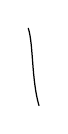
\begin{tikzpicture}[x=1cm,y=1cm,line width=.45pt,line cap=round]
\draw (0,0) .. controls (.065,-.20) and (.040,-.65) .. (.135,-.98);
\end{tikzpicture}}

\uline{N.B.} It should not always be bijective,
for there must be an \inserted{\unsure{outer|outer}} action of a
\(G\) on a \(\widehat{\unsure{\Pi|\pi}}'_0\) i.e. homomorphisms
\(G\longrightarrow\widehat{\widehat{\mathcal T}}(\widehat{\unsure{\Pi|\pi}}'_0)\), which do not \unsure{factor|factor}
through \(\mathcal T(\unsure{\Pi|\pi}'_0)\), and which nevertheless is as
\unsure{good|good} from the profinite group point of view as
\unsure{that|those} coming from a \(\unsure{\Pi|\pi}\) and a \unsure{subgroup}

\scanpage{354}
\mspage{179}

invariant $\unsure{\Pi|\pi}'$. In fact, let us start from such a \uline{discrete} situation $\unsure{\Pi|\pi}_0 \unsure{\supset|>} \unsure{\Pi|\pi}'_0$, whence $G=\unsure{\Pi|\pi}_0/\unsure{\Pi|\pi}'_0$ and $G\longrightarrow \operatorname{Autext}_{\mathrm{lac}}(\unsure{\Pi|\pi}'_0)\deleted{\unsure{(\pi'_0)}}=\mathcal T(\unsure{\Pi|\pi}'_0)\subset\unsure{\widehat{\mathcal T}|\widehat{\widehat{\mathcal T}}}(\widehat{\unsure{\Pi|\pi}}'_0)$, and \uline{conjugate} $G$ by an element \inserted{$\gamma$} of $\widehat{\widehat{\mathcal T}}(\unsure{\Pi|\pi}'_0)$, so as to find $G\longrightarrow\widehat{\mathcal T}(\widehat{\unsure{\Pi|\pi}}'_0)$ which does \deleted{\illegible{2}} not \unsure{factor} through $\mathcal T(\unsure{\Pi|\pi}^{\unsure{'}}_0)$. We find an extension \inserted{$\unsure{\widehat{\unsure{\Pi|\pi}}|\unsure{\Pi|\pi}}^{\unsure{\natural|\sharp}}$} of $G$ by $\widehat{\unsure{\Pi|\pi}}'_0$, \uline{isomorphic} to $\widehat{\unsure{\Pi|\pi}}_0$ (as an extension of $G$ by $\widehat{\unsure{\Pi|\pi}}'_0$), hence the loop structure of $\widehat{\unsure{\Pi|\pi}}'_0$ defines one on $\unsure{\Pi|\pi}^{\unsure{\natural|\sharp}}$ \deleted{and is} \inserted{(so as to be} induced by the latter), but nevertheless the \uline{chosen} discretification \inserted{$\unsure{\Pi|\pi}_0$} of $\widehat{\unsure{\Pi|\pi}}_0$ is not induced by one of $\unsure{\Pi|\pi}$. To

$\ast$ Carry out the construction, it suffices to find an element \inserted{$\gamma\in\widehat{\widehat{\mathcal T}}(\unsure{\Pi|\pi}'_0)$ \deleted{\unsure{finite}} such that $\operatorname{int}(\gamma).G\unsure{\not\subset|\notin}\mathcal T$,} \deleted{\unsure{$u$} \unsure{of order} \illegible{1} not \unsure{coming} from, \unsure{in} $\mathcal T(\unsure{\Pi|\pi}'_0)$, \unsure{or} \unsure{lifting} to an element of finite order of $\unsure{\mathcal G|\mathcal C}(\unsure{\Pi|\pi}'_0)^+=\operatorname{Aut}_{\mathrm{lac}}(\unsure{\Pi|\pi}'_0)^+$, and \deleted{whose \unsure{conjugation} in $\widehat{\widehat{\mathcal T}}$ \unsure{a}} \inserted{a $\gamma\in\widehat{\widehat{\mathcal T}}(\unsure{\Pi|\pi}'_0)$, such that} $\gamma u\gamma^{-1}\notin\mathcal T(\unsure{\Pi|\pi}'_0)$, \inserted{\deleted{i.e. such that $u$ \unsure{fixes}}} \deleted{not} \inserted{$\gamma^{-1}.\unsure{\Pi|\pi}'_0\subset\widehat{\unsure{\Pi|\pi}}'_0$.}}
\figure{[A large part of the canceled passage is enclosed by a frame (left, bottom and right sides) and crossed out with four long slanting strokes. After the inclusion $\gamma^{-1}.\unsure{\Pi|\pi}'_0\subset\widehat{\unsure{\Pi|\pi}}'_0$ on the last line, stroke curved into a hook, directed toward the following inclusion.]}
\inserted{i.e. such that $G$ \deleted{\unsure{does not fix}} does not stabilize $\gamma^{-1}(\unsure{\Pi|\pi}'_0)\subset\widehat{\unsure{\Pi|\pi}}'_0$}

Such a $\gamma$ \unsure{always} exists....

\scanpage{355}

Of course, there is no reason, \deleted{that} for two discretifications $\unsure{\unsure{\Pi|\pi}'_0|\unsure{\Pi|\pi}_0},\unsure{\Pi|\pi}_1$ of $\unsure{\Pi|\pi}$, that if $\unsure{\Pi|\pi}_0,\unsure{\Pi|\pi}_1$ are $\unsure{\Pi|\pi}$-conjugate (i.e. define \deleted{some} \inserted{the same} strict \unsure{prediscretification|prediscretification}\deleted{s} of $\unsure{\Pi|\pi}$), the same should hold for $\unsure{\Pi|\pi}'_0$ and $\unsure{\Pi|\pi}'_1$ under the inner action of $\unsure{\Pi|\pi}'$. (It would be necessary for $\unsure{\Pi|\pi}_0,\unsure{\Pi|\pi}_1$ to be conjugate by $\unsure{\Pi|\pi}'$, and not just by $\unsure{\Pi|\pi}$). On the other hand, I presume that if $\unsure{\Pi|\pi}_0,\unsure{\Pi|\pi}_1$ are ``adherent'' to one another in the space of \unsure{discretifications|discretifications} of $\unsure{\Pi|\pi}$, i.e. if they define the same prediscretification, the same holds for $\unsure{\Pi|\pi}'_0,\unsure{\Pi|\pi}'_1$, and that the map
\[
\tag{4}
\operatorname{Prédiscrt}^{+}(\unsure{\Pi|\pi}\deleted{\unsure{_0}})\longrightarrow\operatorname{Prédiscrt}^{+}(\unsure{\Pi|\pi}'\deleted{\unsure{_0}})
\]
which we obtain in this way, is again bijective, and that it in turn passes to the quotient, to define a bijective map
\[
\tag{5}
\unsure{\operatorname{Préarith}|\operatorname{Préarithm}}(\unsure{\Pi|\pi}\deleted{\unsure{_0}})\longrightarrow\unsure{\operatorname{Préarith}|\operatorname{Préarithm}}(\unsure{\Pi|\pi}'\deleted{\unsure{_0}}),
\]
and that if $\Sigma,\Sigma'$ correspond to one another under the latter, that we have a canonical isomorphism
\[
\tag{6}
\unsure{\mathbb{\Gamma}|\Gamma}_{\Sigma}\longrightarrow\unsure{\mathbb{\Gamma}|\Gamma}_{\Sigma'},
\]
\unsure{compatible},

\scanpage{356}
\mspage{180}

with the actions of these groups on the set $P_{\Sigma}$ of prediscretifications of $\unsure{\Pi|\pi}$ compatible with $\Sigma$, and the set \inserted{$P_{\Sigma'}$} of prediscretifications of $\unsure{\Pi|\pi}'$ compatible with $\Sigma'$ (which are resp. left torsors under $\unsure{\mathbb{\Gamma}|\Gamma}_{\Sigma},\unsure{\mathbb{\Gamma}|\Gamma}_{\Sigma'}$). At the same time, we will find \inserted{therefore} that $\Sigma$ is unique for $\unsure{\Pi|\pi}$ i.e. invariant under $\widehat{\widehat{\mathcal T}}(\unsure{\Pi|\pi})$, iff $\Sigma'$ is unique in $\unsure{\Pi|\pi}'$ i.e. invariant under $\widehat{\widehat{\mathcal T}}(\unsure{\Pi|\pi}')$.

In any case, the fundamental conjecture which \unsure{interprets} the $\unsure{\mathbb{\Gamma}|\Gamma}_{g,\unsure{\nu|v}}$ as $\unsure{\mathbb{\Gamma}|\Gamma}_0=\operatorname{Gal}(\overline{\mathbb Q}_0/\mathbb Q)$ \unsure{would have|will have} at least as a consequence that the map $\operatorname{Discr}^{+}(\unsure{\Pi|\pi})\unsure{-|\longrightarrow}\operatorname{Discr}^{+}(\unsure{\Pi|\pi}')$ passes to the quotient \inserted{in} two ways, to give a commutative diagram

\diagram{
\begin{tikzcd}[row sep=large,column sep=large,ampersand replacement=\&]
\operatorname{Discr}^{+}(\unsure{\Pi|\pi}) \arrow[r,no head] \arrow[d]
  \& \operatorname{Discr}^{+}(\unsure{\Pi|\pi}') \arrow[d] \\
\unsure{P|p}=\unsure{\operatorname{Prédiscr}}^{+}(\unsure{\Pi|\pi}) \arrow[r] \arrow[d]
  \& \unsure{P|p}'=\operatorname{Prédiscr}^{+}(\unsure{\Pi|\pi}') \arrow[d] \\
A=\operatorname{Arithm}(\unsure{\Pi|\pi}) \arrow[r]
  \& A'=\operatorname{Arithm}(\unsure{\Pi|\pi}')
\end{tikzcd}
}

and that the \deleted{\unsure{diagram|diagram}} lower square is cartesian (without prejudging the \unsure{injectivity} or the \unsure{bijectivity} of the map $A\longrightarrow A'$). \unsure{So} it would be necessary